\documentclass{article}
\usepackage[utf8]{inputenc}
\usepackage{import}
\import{.}{preamble.tex}

\title{How to Find a Random Point in a High-Dimensional Ball}
\author{James Zhang}
\date{July 23, 2022}

\begin{document}

\maketitle

\section{Introduction}

Hey everyone, I'm James. Last year, I watched some Summer of Math Exposition videos, and I really enjoyed them, so this year, I'm gonna make one myself.

One of the videos from last year that caught my attention was \href{https://www.youtube.com/watch?v=4y_nmpv-9lI&list=PLnQX-jgAF5pTkwtUuVpqS5tuWmJ-6ZM-Z&index=6&t=3s}{``The BEST Way to Find a Random Point in a Circle"} by Justin. Coincidentally, two of the courses that I took at university this year mentioned higher-dimensional volumes and geometry. So in this video, I'm going to extend Justin's results and talk about how to find a uniform random point in a high-dimensional ball. As you will see, the results in higher dimensions are quite different from those in 2 dimensions.

First of all, let me clarify what I mean by a high-dimensional ball. A ball is a generalization of a circle. A unit circle (and its interior) with radius $r$ is the set of all points $(x, y)$ such that $x^2 + y^2 = r^2$. An $n$-dimensional ball with radius $r$ is the set of all points in $\R^n$ such that $x_1^2 + \ldots + x_n^2 = r^2$.

\section{Rejection Sampling}

The first method that Justin mentioned in his video was rejection sampling. That generalizes easily to $n$ dimensions, so I'm going to implement it. The idea of rejection sampling is that we select a random point from a box, where each coordinate is selected uniformly at random between $-1$ and 1. If the point selected happened to be in the unit ball, we're done. If not, we reject that point and select another one. Let's see how this goes:

\subsection{Python Simulation}

I selected 3141 points for dimensions 1 to 14 and recorded the average number of trials. Here are the results:

% Results from Jupyter Notebook: [1.0, 1.2846227316141356, 1.947787328876154, 3.183381088825215, 6.113976440624005, 12.435848455905763, 27.235275390003185, 62.4157911493155, 155.26774912448266, 404.79337790512574, 1089.8993950971028, 3094.251512257243, 9119.629417383, 28550.63228271251]

\begin{center}
  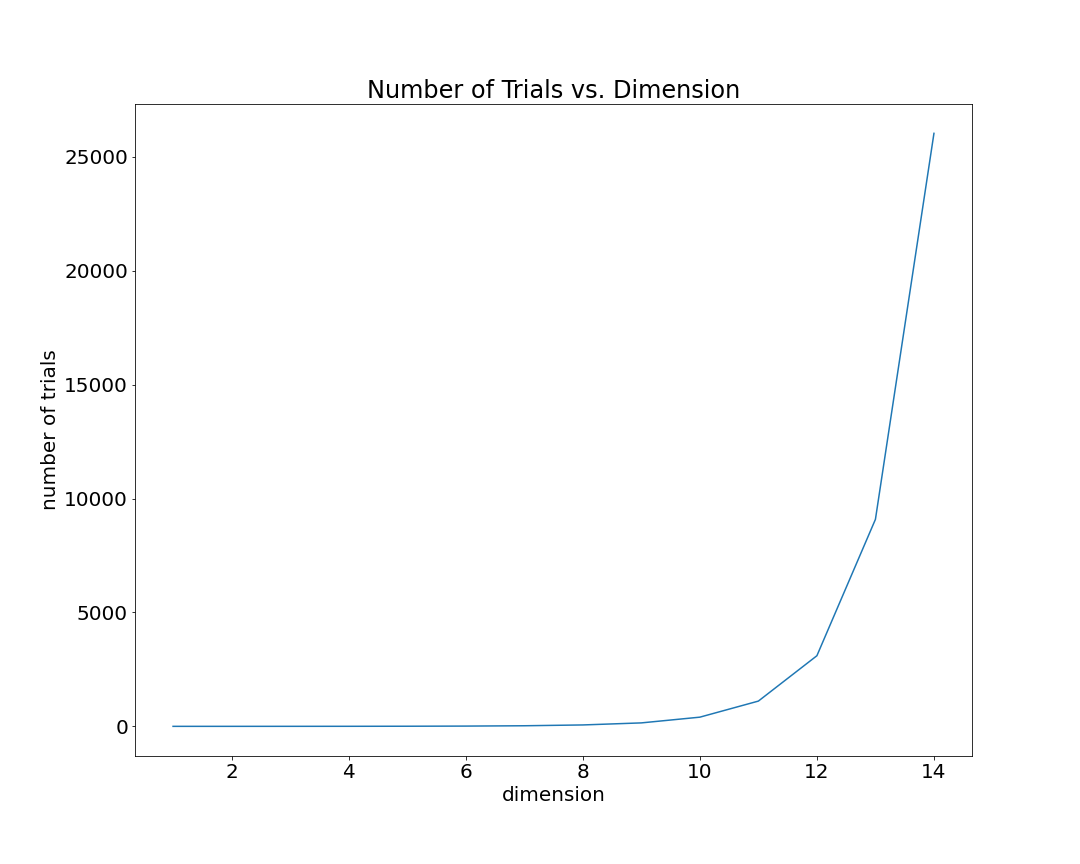
\includegraphics[scale=0.3]{manim/project/images/Trials vs. Dimension Linear.png}
  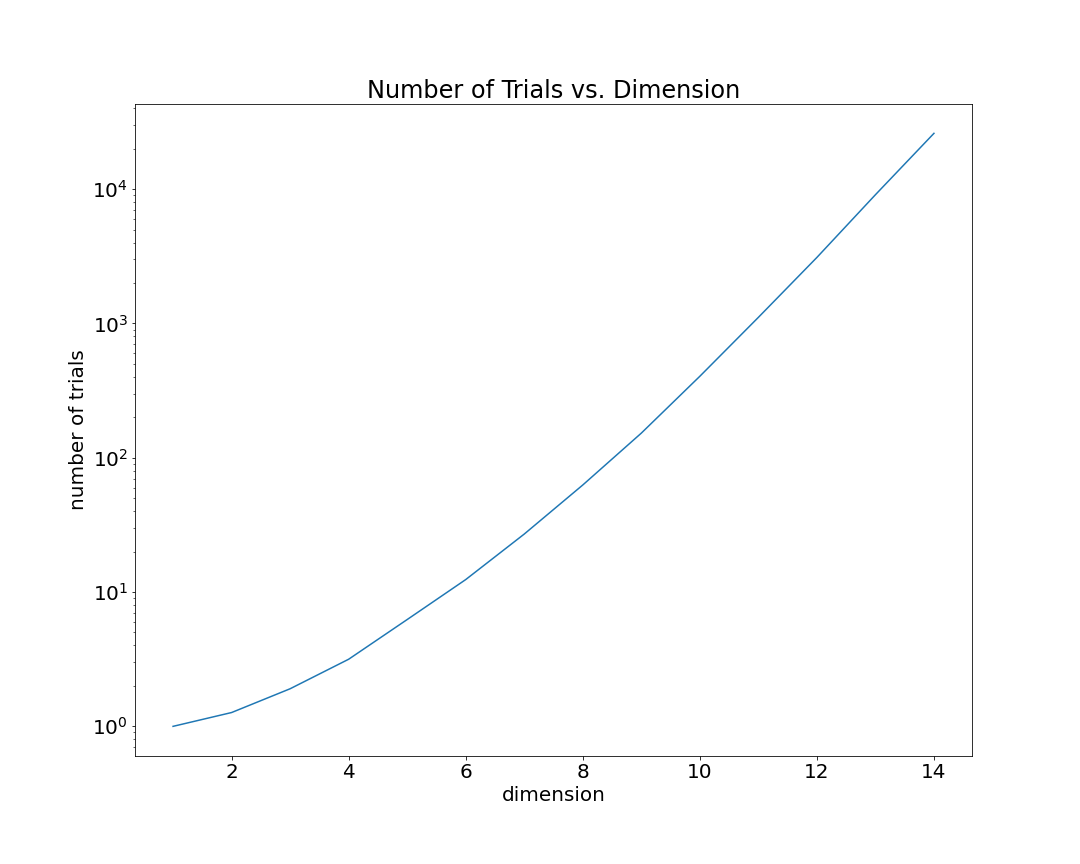
\includegraphics[scale=0.3]{manim/project/images/Trials vs. Dimension Log.png}
\end{center}

As you can see, as the dimension increases, the number of trials increases very rapidly. Even when we switch to log scale for the number of trials, the graph still appears to be concave up. This indicates that the number of trials may grow faster than exponentially with dimension. In 14 dimensions, each point on average requires way over 10,000 trials. We can imagine that in higher dimensions, it takes even more trials. How did that happen?

\subsection{Volume of the Unit Ball}

Let $X$ be the number of trials that we need to select a point in the ball. Since each trial is independent, and we repeat until we succeed, $X$ is a geometric random variable. For any particular trial, the probability that the point we selected is in the ball is equal to the ratio between the volume of the ball and the volume of the box.

Let $\kappa_n$ be the volume of the $n$-dimensional box that we sample from, where $\kappa$ stands for ``cube''. Let $\beta_n$ be the volume of the $n$-dimensional unit ball. Since each component is randomly selected in $[-1, 1]$, the box has side length 2, so its $n$-dimensional volume is $\kappa_n = 2^n$. What about the $n$-dimensional volume of the ball?

% Reference: Vector Calculus, Linear Algebra, and Differential Forms: A Unified Approach by Hubbard & Hubbard

We will use integration and Fubini's Theorem to find out $\beta_n$. We cut the ball into small slices, where the volume of each slice can be approximated by that of a small cylinder. We vary the $x_1$ coordinate from $-1$ to 1 and add up the volumes of the small cylinders. The height of each cylinder is $dx_1$. The base is an $(n-1)$-dimensional ball. In the special case of three dimensions, the base of each slice is a circle.

In general, the radius of the base is $r = \sqrt{1 - x_1^2}$ by the Pythagorean Theorem. Since volume scales appropriately according to dimension, the $(n-1)$-dimensional volume of the base is $r^{n-1} \beta_{n-1}$, where $\beta_{n-1}$ is the volume of the $(n-1)$-dimensional unit ball. Thus,
\[
  \beta_n = \int_{-1}^1 r^{n-1} \beta_{n-1} \, dx_1 = \beta_{n-1} \int_{-1}^1 (1 - x_1^2)^{\frac{n-1}{2}} \, dx_1.
\]

We pulled out $\beta_{n-1}$ from the integral because it is just a constant. It remains to figure out the integral
\[
  c_n = \int_{-1}^1 (1 - t^2)^{\frac{n-1}{2}} \, dt
\]
because then we have the recurrence relation $\beta_n = c_n \beta_{n - 1}$.

Trig substitution with $t = \sin(\theta)$ gives
\begin{align*}
  c_n     & = \int_{-\frac{\pi}{2}}^{\frac{\pi}{2}} \cos^{n}(\theta) \, d\theta   \\
  c_{n-2} & = \int_{-\frac{\pi}{2}}^{\frac{\pi}{2}} \cos^{n-2}(\theta) \, d\theta
\end{align*}

Integration by parts for $c_n$, with $u = \cos^{n-1}(\theta)$ and $dv = \cos(\theta) \, d\theta$ gives

\[
  c_n = \cos^{n-1}(\theta) \sin(\theta) \bigg|_{-\frac{\pi}{2}}^{\frac{\pi}{2}} + \int_{-\frac{\pi}{2}}^{\frac{\pi}{2}} \sin^2(\theta) (n-1) \cos^{n-2}(\theta) \, d\theta
\]

The first term on the right hand side is 0, so
\[
  c_n = (n-1) \int_{-\frac{\pi}{2}}^{\frac{\pi}{2}} \sin^2(\theta) \cos^{n-2}(\theta) \, d\theta
\]

Recall that $\sin^2(\theta) = 1 - \cos^2(\theta)$, so
\[
  c_n = (n-1) \bracks{\int_{-\frac{\pi}{2}}^{\frac{\pi}{2}} \cos^{n-2}(\theta) \, d\theta - \int_{-\frac{\pi}{2}}^{\frac{\pi}{2}} \cos^n(\theta) \, d\theta} = (n-1) c_{n-2} - (n-1) c_n
\]

Rearranging, we get
\[
  c_n = \frac{n-1}{n}c_{n-2}.
\]

The base cases are $c_1 = \int_{-1}^1 (1 - t^2)^0 \, dt = 2$ (by simple integration) and $c_2 = \int_{-1}^1 (1 - t^2)^{\frac{1}{2}} \, dt = \frac{\pi}{2}$ (area of a semicircle). From geometry, we have $\beta_1 = 2$, $\beta_2 = \pi$, $\beta_3 = \frac{4}{3}\pi$.

Recall that $\beta_n = c_n \beta_{n - 1}$. In other words, the ratio between $\beta_n$ and $\beta_{n - 1}$ is $c_n$. If $c_n$ were a constant that is less than 2, say 1.5, then every time we raise a dimension, we double the volume of the box ($\kappa_{n} = 2 \kappa_{n - 1}$), but the volume of the ball only increases by a factor of 1.5. The ratio between the volume of the ball and the volume of the box ($\frac{\beta_n}{\kappa_n}$) will thus decrease by a factor of $\frac{3}{4}$. Since the probability that a particular trial succeeds is equal to that ratio, the probability will decay exponentially by a factor of $\frac{3}{4}$ each time.

However, in reality, $c_n = \frac{n-1}{n}c_{n-2}$, and since $\frac{n-1}{n} < 1$, this means that the multiplier $c_n$ is not a constant: it decreases every time! In fact, there will be an $n$ such that $c_n < 1$, and from that point on, the volume of the ball decreases as we increase dimension. (Here, we're talking about the numerical value of the volume, ignoring the units.)

Therefore, the ratio and thus the probability decays faster than exponentially. Since for a geometric random variable $X$ with success probability $p$, the expected value of $X$ is $\frac{1}{p}$, this implies that the expected number of trials needed to sample a valid point increases faster than exponentially.

\section{Sphere and Distance Method}

Another method to select a random point from a circle that Justin mentioned was to turn to polar coordinates. We first choose $\theta$ uniformly, then choose $r$ so that the points $(r, \theta)$ are distributed uniformly in the circle.

We can try to apply this idea to higher dimensions. In three dimensions, we can try to choose $r, \theta, \vphi$ in some way such that the points represented by $(r, \theta, \vphi)$ in spherical coordinates are distributed uniformly in a three-dimensional ball. However, we can't choose $\vphi$ uniformly because when $\vphi$ is close to $\frac{\pi}{2}$, that is, we're choosing points near the equator, we expect to see way more points than when $\vphi$ is close to 0 or $\pi$ (or near the poles). There are higher-dimensional analogs of the spherical coordinates in higher dimensions, but we can imagine that as the dimensions go up, it would be increasingly difficult to keep track of the distributions of each variable.

Instead, we take a similar approach: First choose a direction uniformly at random, and then choose a random number between 0 and 1 to be the distance from the origin.

Choosing a random direction in n-dimensional space is the same as choosing a random point on the n-dimensional unit sphere. A sphere is the boundary of a ball, and points on the unit sphere satisfy $x_1^2 + \ldots + x_n^2 = 1$.

So now, our task is divided into two parts: Choosing a random point on the unit sphere and choosing a distance from the origin. We'll focus on the first part for now and worry about choosing a distance later.

\subsection{Random Point on Sphere}

\subsubsection{Failed Attempt}

The first way that comes to mind is this: We choose a random vector from the box $[-1, 1]^n$ where each component is chosen uniformly in $[-1, 1]$. Then we normalize this vector by dividing away its length. The resulting vector is a unit vector, so it lies on the unit sphere.

This seems like a good approach, but after some thought, we can see that the random points generated in this way aren't distributed uniformly on the sphere. Intuitively, It is more likely to choose a point near the diagonals of the box than near the center of the faces. Let's look at a two-dimensional example:

% Draw picture of square

The distance from the origin to the upper-right corner is $\sqrt{2}$, whereas the distance from the origin to the upper edge is 1. Consider these two cones, which are just triangles in 2D. If a random vector falls into the green cone, it will be scaled to a point on this green arc. If a random vector falls into the blue cone, it will be scaled to a point on this blue arc. The cones are drawn such that the blue and the green arcs have the same length. Then these two cones are similar, and the ratio between their areas is $\parens{\frac{\sqrt{2}}{1}}^2$.

For $n$ dimensions, the diagonal distance will be $\sqrt{n}$ times larger, and the ratio between the volumes of the cones will be $\parens{\frac{\sqrt{n}}{1}}^n$. This again grows faster than exponentially, which means that the probability that a random point lands on one region of the sphere is more than exponentially bigger than the probability that a random point lands on some other region of the sphere with the same area.

\subsubsection{Rotational Invariance and the Multivariate Normal Distribution}

The problem with the box is that it is not rotationally invariant: If we rotate the box by a certain amount, the rotated box doesn't look the same as the original. Meanwhile, the ball and the sphere are all rotationally invariant: However we rotate them, they look the same.

Every rotation in $\R^n$ can be characterized by an orthogonal matrix. An orthogonal matrix is a matrix whose columns (and rows) form an orthonormal basis. (Note: All rotations are isometries, but not all isometries are rotations.) For instance, in $\R^2$, we can express a rotation like this:
\[
  Q = \begin{bmatrix}
    \cos(\theta) & -\sin(\theta) \\
    \sin(\theta) & \cos(\theta)
  \end{bmatrix}
\]

The columns $\xymatrix{\cos(\theta)}{\sin(\theta)}$ and $\xymatrix{-\sin(\theta)}{\cos(\theta)}$ are orthonormal because the length of both vectors are
\[
  \sqrt{\cos^2(\theta) + \sin^2(\theta)} = 1
\]
and the dot product between the two vectors is 0. Similarly, the rows of $Q$ are also orthonormal.

% Manim rotation animation

To figure out a valid way to choose a point uniformly on the sphere, we need to think outside the box. Literally. Introducing the multivariate normal distribution. As you might know, the probability density function of a normal random variable is shaped like a bell curve. Here, we're using the standard multivariate normal distribution, denoted $\mathcal{N}(\mathbf{0}, I)$, which is a vector of independent random variables, where each component follows the standard normal distribution $\mathcal{N}(0, 1)$. (Here I'm using ``normal'' and ``Gaussian'' interchangeably.)

You might also know that any linear combination of independent normal random variables is still a normal random variable. We can use this fact to show that the standard multivariate normal distribution is rotationally invariant:

Suppose $Q$ is the orthogonal matrix representing an arbitrary rotation in $\R^n$, and
$X = \begin{bmatrix}
    X_1 \\ \vdots \\ X_n
  \end{bmatrix}$ is a standard multivariate normal. Then each $X_i$ is a Gaussian with mean 0 and variance 1.

Let $q_{1,1}, \ldots, q_{1,n}$ be the first row of $Q$. Then the first element of $QX$ is $Y_1 = q_{1,1} X_1 + \ldots + q_{1,n} X_n$. Since $Q$ is orthogonal, $q_{1,1}^2 + \ldots + q_{1,n}^2 = 1$.

Since the $X_i$'s are independent Gaussian random variables, the linear combination is still a Gaussian random variable. Moreover, by linearity of expectation, the mean of $Y_1$ is $\mu(Y_1) = q_{1,1} \mu(X_1) + \ldots + q_{1,n} \mu(X_n) = 0$, and by independence, the variance of $Y_1$ is $\Var(Y_1) = q_{1,1}^2 \Var(X_1) + \ldots + q_{1,n}^2 \Var(X_n) = q_{1,1}^2 + \ldots + q_{1,n}^2 = 1$.

We have shown that $Y_m$ is a normal random variable. This is the same for each element of $Y = QX$, so $Y$ is still a standard multivariate normal. Thus $X$ is rotationally invariant.

Here's a graph of the joint density function of a 2-dimensional standard multivariate normal random variable. We can see from the density function that the distribution is indeed symmetric around the origin.

\begin{center}
  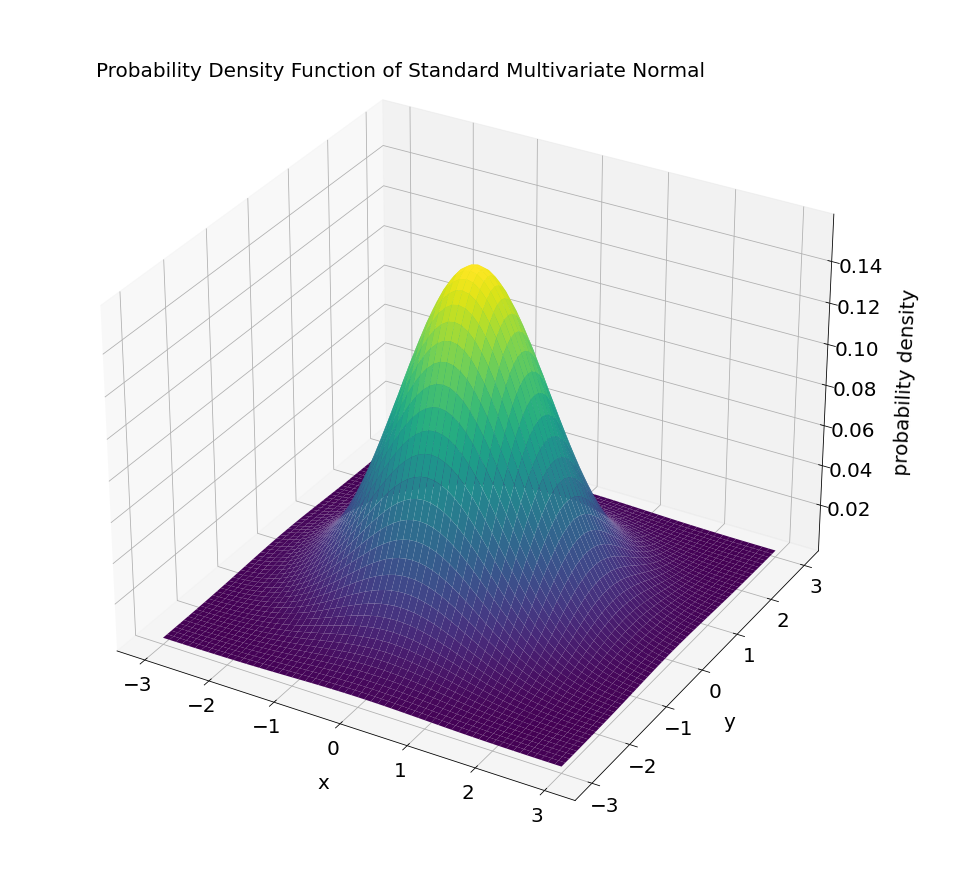
\includegraphics[scale=0.3]{manim/project/images/Multivariate Normal PDF.png}
\end{center}

Now, we can first generate a random vector that follows the multivariate normal distribution and normalize it, and it will give a point on the unit sphere selected uniformly at random. To see why it is uniform, choose two different small patches of the sphere, $A$ and $B$, that are congruent to each other. Suppose that $p$ is the probability that a random unit vector chosen above falls in $A$. Then we can rotate the sphere so that $A$ coincides with $B$. Thus the probability that a chosen vector falls in $B$ after the rotation is $p$. Because the multivariate normal distribution is rotationally invariant, the distribution of points after the rotation is the same as the distribution before the rotation, so the probability that a random unit vector falls in $A$ after the rotation is also $p$.

There is still the problem of how to generate a Gaussian random variable from a uniform random variable. This is a good topic for a separate video, and I'm just going to rely on the python library to do this, but for those who are interested, there is an algorithm called the Box-Muller Transform which does just that. The key feature of that algorithm is that it runs in polynomial time.

\subsection{Choosing the Distance}

After finding a uniformly random point on the sphere, it's now time to choose the distance from the origin. Here, we use the same method as Justin used in his video. Let $R$ be the random variable that denotes the distance from the origin. We first find the cumulative distribution function (CDF) $F_R$, where $F_R(r)$ is the probability that $R \leq r$.

The set of all points with distance to the origin less than or equal to $r$ form a ball of radius $r$. The probability that $R \leq r$ is thus the ratio between the volume of a ball of radius $r$ and the unit ball. Since volumes scale appropriately according to dimension, that ratio is $\parens{\frac{r}{1}}^n$. Thus, $F_R(r) = r^n$.

Notice how for a given $r \in (0, 1)$, as $n$ increases, the probability that $R \leq r$ gets smaller and smaller. This implies that as $n$ increases, most of the volume of the ball concentrates near the surface of the ball. For instance, when $n = 500$, the probability that a random point in the unit ball is at least 0.99 units away from the origin is $99.3\%$.

Now we shall use the Inverse Transform Sampling technique that Justin mentioned: If $U$ is a uniform random variable, then $R$ has the same distribution as $F_R^{-1}(U)$. In our case, we have $R = \sqrt[n]{U}$.

\subsection{Python Simulation}

Here's my python code that generates random points in unit balls using this process. Notice that even when $n$ is big, the program still finds random points in $n$-dimensional unit balls very quickly. Unfortunately, I cannot plot higher-dimensional points in our 3D world, so here's a demonstration of this algorithm in 2 and 3 dimensions.

% Manim animation for 2 and 3 dimensions

\section{Reflection}

\section{Acknowledgements}

\begin{itemize}
  \item Justin's video: \href{https://www.youtube.com/watch?v=4y_nmpv-9lI&list=PLnQX-jgAF5pTkwtUuVpqS5tuWmJ-6ZM-Z&index=6&t=3s}{``The BEST Way to Find a Random Point in a Circle"}
  \item \textit{Vector Calculus, Linear Algebra, and Differential Forms: A Unified Approach} by John Hubbard and Barbara Burke Hubbard
  \item \textit{Foundations of Data Science} by Avrim Blum, John Hopcroft, and Ravindran Kannan
  \item \textit{Introduction to Probability} by David F. Anderson, Timo Sepp\"{a}l\"{a}inen, and Benedek Valk\'{o}
  \item \href{https://scipython.com/blog/visualizing-the-bivariate-gaussian-distribution/}{This website} helped me generate the graph of the PDF of the standard multivariate normal
\end{itemize}

\end{document}
